% !TEX root = ../thesis.tex

CORE builds on three key components---MDE, model reuse, and Separation of Concerns (SoC)---to support large-scale model reuse. In this chapter, we provide an overview of CORE as a reuse technique with the current state of development in Section~\ref{sec:2.1}. Since we are also interested in studying the early phases of software development, where the requirements of the software to be built are established, we describe UCM as part of the requirements modeling tool and its use in specifying scenarios in Section~\ref{sec:2.2}. We then survey on existing aspect-oriented modeling techniques related to our work in Section~\ref{sec:2.3}.

\section{Concern-Oriented Reuse (CORE)} \label{sec:2.1}

CORE is a reuse technique that extends MDE with best practices from advanced modularization and SoC techniques~\cite{dijkstra1976discipline}, as well as features and goal modeling to support SPL~\cite{pohl2005software}. Variations exist for any given solution, and creating a collection of similar software systems from a shared set of software artifacts to support SPL is possible through software reuse. MDE, reuse, and SoC form the three fundamental principles of CORE.

The objective of MDE is to develop software through modeling, where models are built using the formalisms that best describe and encapsulate the relevant properties for each level of abstraction. Through model transformations, models at high levels of abstraction can be integrated with solution-specific models at lower levels of abstraction. This process continues until a final model, which may be executable, is generated. CORE uses these concepts, especially the ability of MDE to embed domain-specific knowledge into models, to bridge the gap between domain and system knowledge.

The aim of reuse is to develop software by reusing existing software artifacts instead of creating them from scratch. Software reuse results in a hierarchy of reusable artifacts, where smaller reusable artifacts are integrated to form increasingly larger reusable artifacts. To make software reuse applicable, reusing an artifact should be easier than constructing it from scratch. This entails that the reusable artifacts are easy to understand, find, and apply~\cite{coulange2012software, krueger1992software}. Benefits of reuse include increase in productivity and maintainability, as well as reduction in cost and time-to-market.

The third foundation of CORE is based on the ideas of SoC and information hiding~\cite{dijkstra1976discipline, parnas1972criteria}. When concerns are well-separated, individual sections can be reused, optimized independently, and insulated from potential failures of other sections. Multi-dimensional SoC provides the ability to separate overlapping concerns and further extends SoC by defining a conceptual framework where concerns are treated as first-class entities during software development~\cite{tarr1999n}.

In the next subsection, we describe in detail how CORE enables reuse hierarchies through the three interfaces that a CORE concern provides, and formalize the key concepts of CORE for each interface in the CORE metamodel.

\subsection{Concern Reuse Process}

\begin{figure}
	\centering
	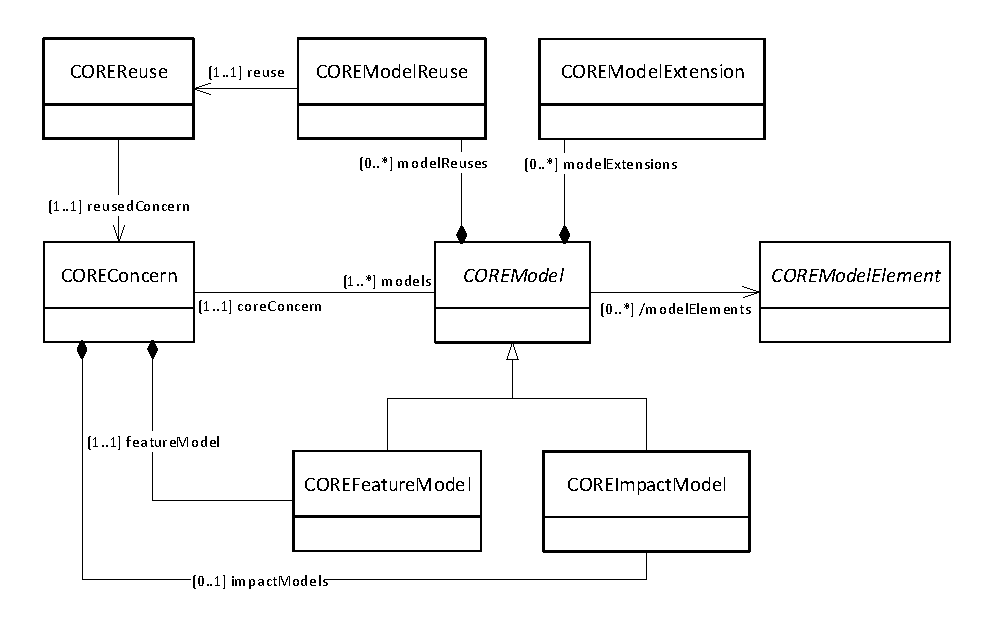
\includegraphics[scale=0.65]{fig_2_1.pdf}
	\caption{CORE metamodel: basic structure of a concern}
	\label{fig:2.1}
\end{figure}

A CORE concern consists of a feature model, an optional impact model, and various realization models. The features in a feature model affect stakeholder goals that are expressed with the impact model, while realization models characterize the features.

Figure~\ref{fig:2.1} formalizes the key concepts for the basic structure of a concern (see Figure~\ref{fig:a.1} in Appendix~\ref{ch:A} for the complete CORE metamodel). A concern ({\cls COREConcern}) groups related models (\textit{\cls COREModel}) together and provides at least one model by default---a feature model ({\cls COREFeatureModel}; subclass of \textit{\cls COREModel}). Additionally, a concern may have an optional impact model ({\cls COREImpactModel}; subclass of \textit{\cls COREModel}) and several realization models that subclass \textit{\cls COREModel} defined by a corified \footnote{The term \emph{corify} (verb: \textbf{corify}; past participle: \textbf{corified}; present participle: \textbf{corifying}; noun: \textbf{corification}) means to integrate a modeling language with CORE.} modeling language (not shown in Figure~\ref{fig:2.1}). A \textit{\cls COREModel} groups related model elements (\textit{\cls COREModelElement}).

A concern can reuse other concerns, which results in a simple reuse hierarchy consisting of two concerns, with the reused concern and the reusing concern having the same internal structure. A reusing concern has a {\cls COREReuse} associated to the reused concern, and reusing a concern entails reusing its models. Consequently, a {\cls COREModelReuse} is defined for each model of the concern that is reused. In addition, reuse also occurs within a concern, namely the extension of a feature ({\cls COREModelExtension}), because the realization models of one feature may reuse the realization models of another feature.

The concern reuse process offers three interfaces to facilitate reuse~\cite{alam2013concern}. The variation interface presents the design alternatives and their impact on non-functional requirements. The customization interface of the selected alternative details how to adapt the generic solution to a specific context. Finally, the usage interface specifies the provided behavior. These three interfaces allow a concern user to reuse a concern by following the simple three-step process outlined below.

\subsubsection{Step 1: Variation Interface}

The variation interface describes the possible variations of the concern and the impact of different variants on high-level stakeholder goals, system qualities, and non-functional requirements. The variations are represented with a feature model~\cite{kang1990feature} that specifies the individual features that a concern offers as well as their dependencies. The impact model represents the impact of choosing a feature and can be specified with goal models using GRL, which is part of the URN standard~\cite{itu2012151}.

A feature model captures the potential features of members of an SPL in a tree structure, containing those features that are common to all members and those that vary from one member to the next. A particular member is defined by selecting the desired features from the feature model, resulting in a feature model configuration~\cite{czarnecki2005staged}. Inter-feature relationships allow the specification of (i) mandatory and optional parent-child feature relationships as well as (ii) exclusive (XOR) and alternative (IOR) feature groups. A mandatory parent-child relationship specifies that the child is included in a feature model configuration if the parent is included. In an optional parent-child relationship, the child does not have to be included if the parent is included. Exactly one feature must be selected in an XOR feature group if its parent feature is selected, whereas at least one feature must be selected in an IOR feature group if its parent feature is selected.

In Step~1 of the CORE reuse process, the concern user must first select the feature(s) with the best impact on relevant stakeholder goals and system qualities from the variation interface of the concern based on provided impact analysis~\cite{duran2016investigation}. To maximize the reusability of the concern that is being built, the user should select from the reused concern only the features that are absolutely necessary to achieve the required functionality and goals. Decisions about potential use of alternative or optional features should be delayed by reexposing them~\cite{kienzle2016delaying}. Based on a configuration, the CORE modeling tool composes the generic realization models of each modeling language that realize the selected features to yield new, user-tailored realization models of the concern corresponding to the desired configuration. Depending on the root phase of the concern, this composition may involve requirement models, architecture models, design models and/or code.

\begin{figure}
	\centering
	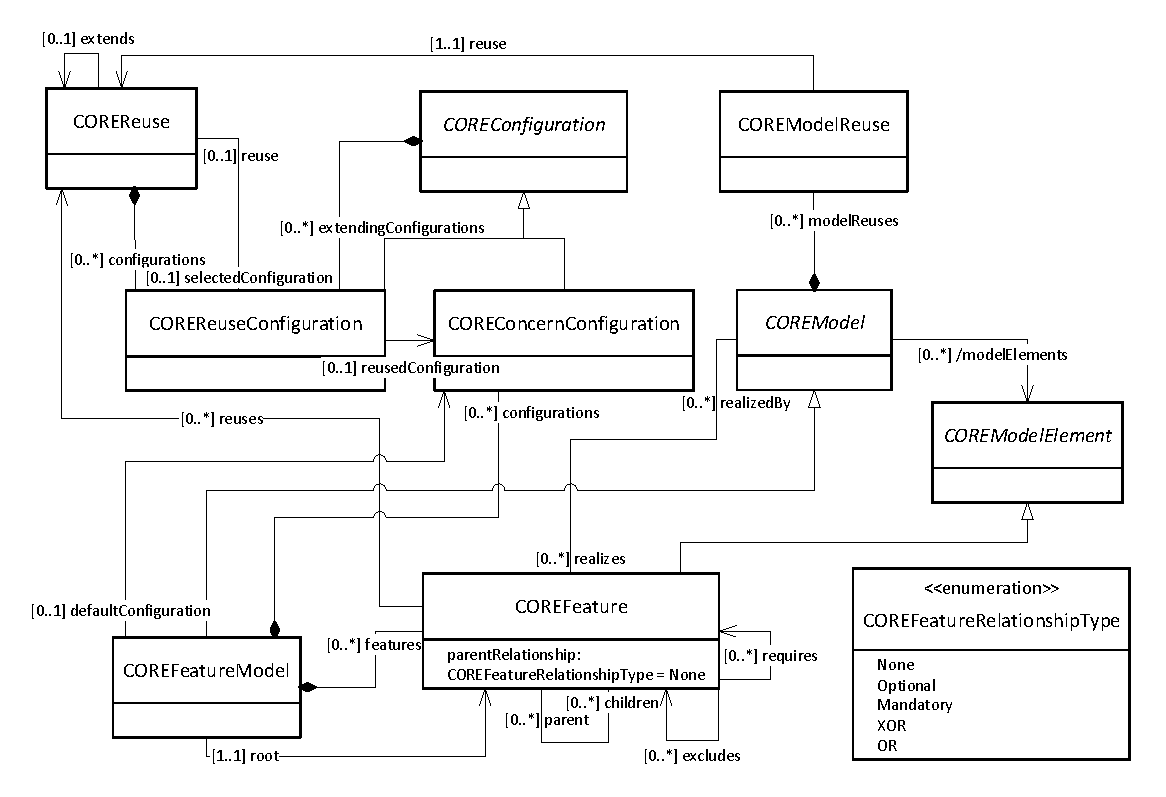
\includegraphics[scale=0.65]{fig_2_2.pdf}
	\caption{CORE metamodel: variation interface - features}
	\label{fig:2.2}
\end{figure}

The metamodel excerpt in Figure~\ref{fig:2.2} describes the part of the variation interface of CORE related to the feature model. A feature ({\cls COREFeature}) is contained in {\cls COREFeatureModel}. Exactly one feature is the \emph{root} feature of the feature model. {\cls COREFeature} has an attribute (\emph{parentRelationship}), which is an enumeration of {\cls COREFeatureRelationshipType}, that specifies the relationship of a feature with its parent. Possible relationships include whether the feature is part of an \emph{XOR} or \emph{OR} group; whether it is \emph{Mandatory} or \emph{Optional}; or whether it is the root (\emph{None}). A feature selection may \emph{require} or \emph{exclude} the selection of other features. Each feature has at most one \emph{parent} and may have many \emph{children}. A feature may be \emph{realizedBy} many \textit{\cls COREModel}s, and similarly,\textit{\cls COREModel} may \emph{realize} many features. This association is used to link features to the models of the corified modeling language. Furthermore, a configuration (\textit{\cls COREConfiguration}) defines the \emph{selected} and \emph{reexposed} features. A feature model may predefine several commonly used \emph{configurations}, one of which may be designated as the \emph{defaultConfiguration}. A {\cls COREReuse} defines its own \emph{configurations}, one of which may be designated as the \emph{selectedConfiguration}. This allows configurations of the reused concern to be modified according to changes in the reuse context. A configuration of a {\cls COREReuse} may either directly select and reexpose features of the reused concern, or it may choose one of the predefined configurations (\emph{reusedConfiguration}) of the reused concern and optionally select and reexpose additional features.

In addition to the feature model, the impact model is also part of the variation interface that helps the user perform trade-off analysis when selecting the features. Goal models are used for impact analysis because of the ability to allow vague, hard-to-measure system qualities to be evaluated, in addition to more quantifiable qualities. Goal modeling is typically applied in early requirements engineering activities to capture stakeholder and business objectives, alternative ways of satisfying these objectives, and the positive/negative impacts of these alternatives on various high-level goals and quality aspects. The analysis of goal models guides the decision-making process, which seeks to find the best suited alternative for a particular situation. These principles also apply in the CORE context, where an impact model is a type of goal model that describes the advantages and disadvantages of features offered by a concern and gives an indication of the impact of a selection of features on high-level goals that are important to the concern user. The goal model for the variation interface is called impact model to signify that goal models in CORE are different from traditional goal models---not only because the main focus is on capturing the impact of features on qualities, but their use is more restricted and specialized. Impact models use features in place of tasks, and they use relative quantitative contributions exclusively to express the impact on goals of importance for the concern~\cite{duran2015reuse}.

Similar to the feature model, the impact model is also reused by reconnecting the impact model of the reusing concern with the impact model of the reused concern. This allows for system-wide trade-off analysis and is accomplished by a feature impact node. The feature impact node expresses (i) that an impact only occurs if the feature is selected, (ii) which reused concerns impact the goal in the context of the feature, and (iii) how much the feature itself and the reused concerns contribute to the goal.

\begin{figure}
	\centering
	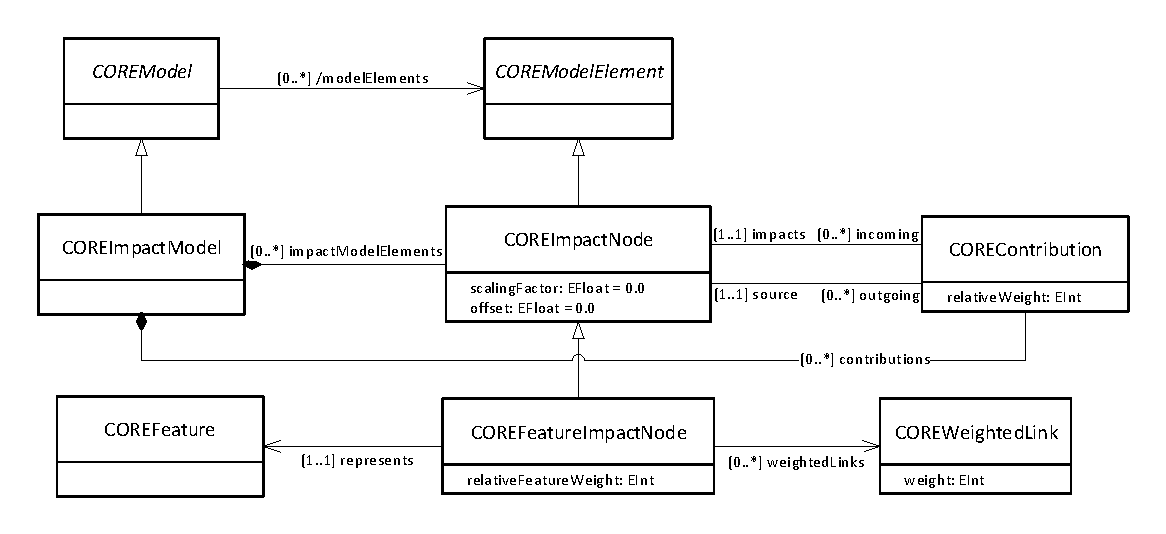
\includegraphics[scale=0.65]{fig_2_3.pdf}
	\caption{CORE metamodel: variation interface - impacts}
	\label{fig:2.3}
\end{figure}

The metamodel excerpt in Figure~\ref{fig:2.3} describes the part of the variation interface of CORE related to the impact model. A {\cls COREImpactModel} contains both nodes ({\cls COREImpactNode}s) and contributions ({\cls COREContribution}s). A goal is represented by a {\cls COREImpactNode} (a subclass of \textit{\cls COREModelElement}). Its \emph{scalingFactor} and \emph{offset} are used by the normalization step to ensure that the satisfaction value of a node is always between 0 and 100. On the other hand, any {\cls COREFeature} is represented by a {\cls COREFeatureImpactNode} (a subclass of {\cls COREImpactNode}) in the impact model. Each {\cls COREContribution} has a \emph{relativeWeight} integer attribute to store its contribution value, describing how one {\cls COREImpactNode} (\emph{source} role) impacts another {\cls COREImpactNode} (\emph{impact} role). If a feature makes use of a reused concern, then the impact of a {\cls COREFeatureImpactNode} relative to the impact of the reused concern is described by its \emph{relativeFeatureWeight} and the \emph{weight} of its {\cls COREWeightedLink} that represents the impact of the reused concern used by the feature~\cite{duran2015evaluation, alexandre2015support}. A {\cls COREFeatureImpactNode} is created for each goal that is impacted by the feature. A {\cls COREWeightedLink} exists for each reused concern used by the feature that impacts the goal.

\subsubsection{Step 2: Customization Interface}

The customization interface describes how a chosen variant can be adapted to the needs of a specific application. Each variant of a concern is described as generally as possible to increase reusability. Therefore, some elements in the concern are only partially specified and need to be related or complemented with concrete modeling elements of the application that intends to reuse the concern. The customization interface is hence used when a specific variant of a reusable concern is composed with the application.

In Step~2 of the reuse process, the concern user has to adapt the generated user-tailored, yet still generic, realization models of the concern to the application context by mapping elements from the customization interface to elements from the application context. Depending on the root phase of the concern, this step might require customizing requirement models, architecture models, design models, and/or code. Based on the customization mappings, the CORE tool then composes the user-tailored concern realization models with the application-specific models to yield adapted realization models of the concern.

\begin{figure}
	\centering
	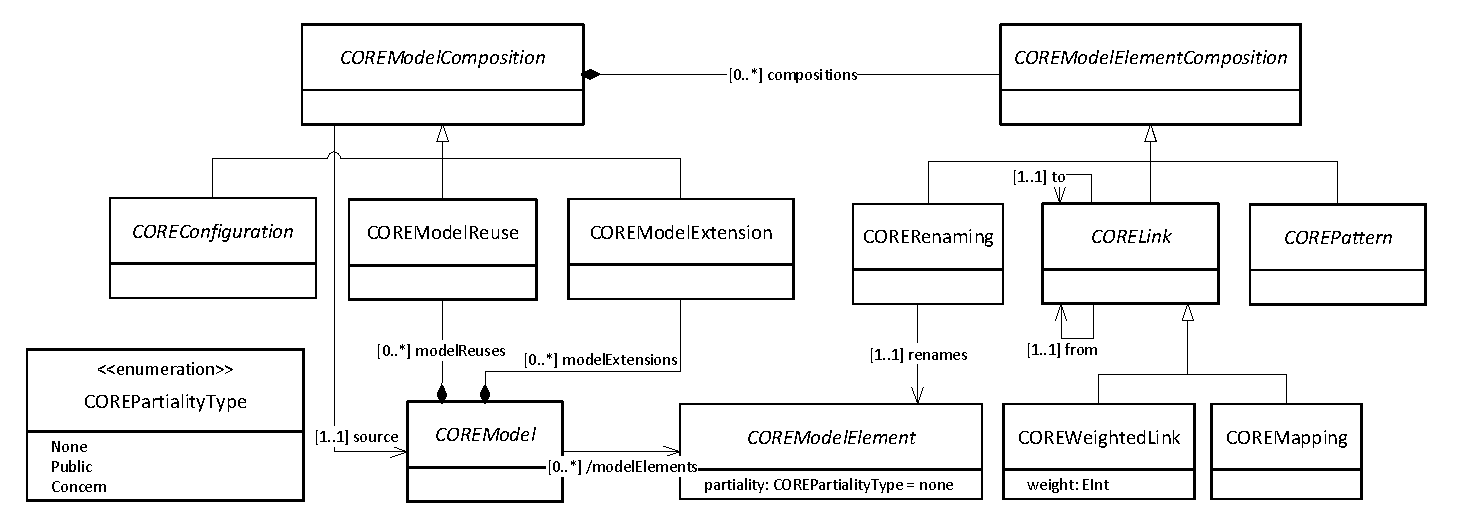
\includegraphics[scale=0.65]{fig_2_4.pdf}
	\caption{CORE metamodel: customization interface}
	\label{fig:2.4}
\end{figure}

The customization interface manifests itself in the metamodel excerpt shown in Figure~\ref{fig:2.4} by the \emph{partiality} attribute of \textit{\cls COREModelElement}. A model element must be adapted either by a reusing concern (\emph{Public}), by another feature in the same concern (\emph{Concern}), or not at all (by default \emph{None}; it is not a generic element).

The remaining metaclasses provide the means to compose an element in the customization interface with an element from the reusing concern. The type of composition (\textit{\cls COREModelComposition}) depends on the model that needs to be composed. \textit{\cls COREModelComposition} captures the fact that all compositions combine a \emph{source} (i.e., reused model) with the reusing model and that several elements of the model may have to be composed (\textit{\cls COREModelElementComposition}). \textit{\cls COREConfiguration} is dedicated to the composition of feature models (discussed in Step~1 of the reuse process). \textit{\cls COREModelElementComposition}s are not needed for feature models, but the other two concrete subclasses of \textit{\cls COREModelComposition}---{\cls COREModelReuse} and {\cls COREModelExtension}---do require \textit{\cls COREModelElementComposition}s. \textit{\cls COREModelElementComposition} has two abstract subclasses---\textit{\cls CORELink} and \textit{\cls COREPattern}---representing two general ways for specifying compositions for modeling languages other than feature models~\cite{mussbacher2012assessing, alam2013revising}. \textit{\cls COREPattern} is used when the composition is specified using pattern matching, while \textit{\cls CORELink} is used when a pair of \textit{\cls COREModelElement}s is composed. The \emph{from} element always refers to a model element from the reused concern while the \emph{to} element refers to a model element from the reusing concern. The subclasses of \textit{\cls CORELink} differentiate weighted ({\cls COREWeightedLink}; used for impact models and discussed in Step~1 of the reuse process) and non-weighted mappings ({\cls COREMapping}). In total, there are three different techniques for composing model elements covered by the CORE metamodel.

\subsubsection{Step 3: Usage Interface}

The usage interface describes how the application can finally access the structure and behavior provided by the concern. While one variation interface consisting of feature and impact models exists for the whole concern, the customization interface and usage interface typically exist for each other type of model/modeling language used to realize the functionality encapsulated within the concern (i.e., for each corified modeling language).

In Step~3 of the reuse process, the concern user can then use the functionality provided by the selected concern features that are exposed in the usage interface of the adapted realization models within the user's own application models.

\begin{figure}
	\centering
	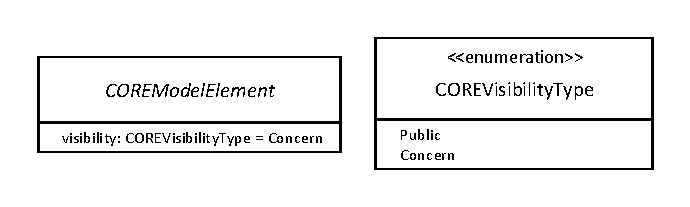
\includegraphics[scale=0.65]{fig_2_5.pdf}
	\caption{CORE metamodel: usage interface}
	\label{fig:2.5}
\end{figure}

The usage interface manifests itself in the metamodel excerpt shown in Figure~\ref{fig:2.5} by the \emph{visibility} attribute of {\cls COREModelElement}. A model element can either be accessed by a reusing concern (\emph{Public}) or is only visible within a concern (\emph{Concern}).

\subsection{CORE Weaver}

As explained in Step~1 of the reuse process, after the user selects the desired features of the reused concern, the modeling tool composes the realization models of the selected features to yield a realization of the concern that only contains the features that the user intends to use. This subsection describes the weaving process that flattens an entire concern hierarchy given a specific configuration to generate a final realization model where all involved concerns are merged. The process of model composition utilizes the weaver that weaves recursively by traversing the concern hierarchy, as illustrated in detail by Kienzle et al.~\cite{kienzle2016delaying}, in which the composition algorithms support delayed decision making in CORE. Each corified modeling language has its own weaver to compose a particular model as different models require specific algorithm for composition. Nonetheless, CORE has a generic weaver that administers model composition to the appropriate weaver. The CORE weaver performs either a \emph{single weave} or \emph{complete weave}.

\textbf{Single Weave:} This process weaves two directly dependent models together. This is the fundamental unit of weaving as model composition of a concern begins with this step. Model elements are copied from the lower-level/mode generic model to the higher-level/more specific model within a concern prior to composition, and references of elements need to be updated post-composition based on the information of elements mapped from lower-level model to higher-level model.

\textbf{Complete Weave:} This process weaves all dependent models of a concern hierarchy, forming an independent model that represents the merged models from the selected features of a concern. The weaver first selects the pair of models that has the highest depth level in the concern (tree), reducing the pair of models into a woven model through \emph{single weave}. This is carried on recursively until the weaver resolves all dependencies, resulting in a final woven model once there are no dependencies left.

\section{Use Case Maps (UCM)} \label{sec:2.2}

UCM is a visual notation that aims to link behavior and structure of a system~\cite{amyot2003introduction, buhr1995use}. UCM paths are first-class architectural entities that describe causal relationships between responsibilities that may be bound to underlying organizational structures of abstract components~\cite{buhr1998use}. UCMs are used to describe and integrate use cases representing the requirements, and UCM paths represent scenarios that intend to bridge the gap between requirements and detailed design.

\begin{figure}
	\centering
	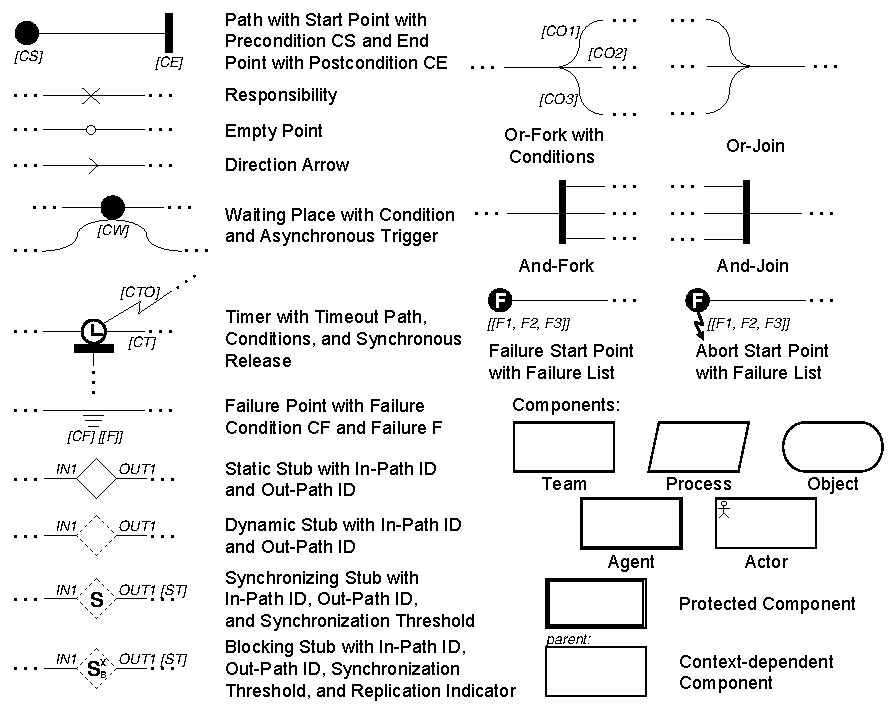
\includegraphics[scale=0.9]{fig_2_6.pdf}
	\caption[UCM notation]{UCM notation. Image courtesy of ITU~\cite{itu2012151}}
	\label{fig:2.6}
\end{figure}

Figure~\ref{fig:2.6} illustrates the basic elements of the UCM notation. A map contains any number of paths and optionally components. Paths express causal sequences and may contain several types of path nodes, each linked with \emph{node connections} (wiggly lines). Paths begin at \emph{start points} (filled circles---representing preconditions or triggering causes) and terminate at \emph{end points} (bars---representing postconditions or resulting effects). \emph{Responsibilities} (crosses---representing actions, tasks, or functions to be performed) describe required actions or steps to fulfill a scenario. Alternatives are represented as overlapping paths. An \emph{OR-fork} splits a path into multiple alternatives, while an \emph{OR-join} merges multiple overlapping paths. Alternatives may be guarded by conditions represented as labels between square brackets. On the other hand, concurrent routes are represented through the use of vertical bars. An \emph{AND-fork} splits a path into multiple concurrent segments, while an \emph{AND-join} synchronizes multiple paths together. Other notational elements include \emph{waiting places} (filled circles---representing synchronous or asynchronous interactions), \emph{timers} (clocks---representing waiting places triggered by timely arrival of specific events), \emph{aborts} (zigzag lines---representing paths that terminates the execution of other causal chain of responsibilities), and \emph{failure points} (ground symbols---representing potential failure points on a path).

A map that is too complex to be represented in a single UCM model can be decomposed into sub-maps. A top-level UCM, referred to as a root map, can include containers (called \emph{stubs}) for sub-maps (called \emph{plug-ins}). \emph{Plug-in bindings} define the continuation of a path between stubs and plug-ins, by connecting the path segments coming in and going out of a stub with start and end points of the plug-ins. A stub of kind \emph{static} (plain diamond) can only contain at most one plug-in, whereas a stub of kind \emph{dynamic} (dashed diamond) may contain several plug-ins. A \emph{selection policy} (often described with preconditions) determines which plug-ins of a dynamic stub to choose from during runtime. A stub of kind \emph{synchronizing} (dashed diamond with symbol S) is a dynamic stub that allows its plug-ins to be executed in parallel and continues only once the plug-ins have synchronized. Finally, a stub of kind \emph{blocking} (dashed diamond with symbol S\textsubscript{B}) is a synchronizing stub that does not allow its plug-ins to be visited more than once at the same time.

\begin{figure}
	\centering
	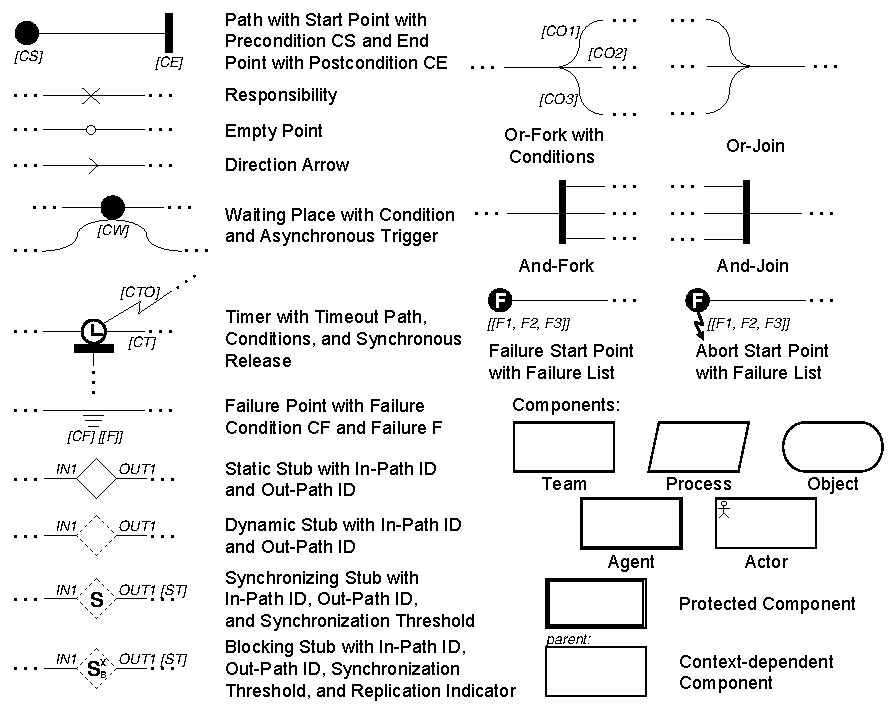
\includegraphics[scale=0.9]{fig_2_7.pdf}
	\caption[UCM metamodel]{UCM metamodel. Image courtesy of ITU~\cite{itu2012151}}
	\label{fig:2.7}
\end{figure}

Components are used to specify the structural aspects of a system. A responsibility is bound to a component when the cross is inside the component. As such, the component is responsible for performing the action, task, or function represented by the responsibility. Components can be of different kinds, have various attributes, and may contain sub-components. For example, a component of kind \emph{object} (rounded rectangle) represents a passive component that does not have its own thread of control, while a component of kind \emph{process} (parallelogram) represents an active component that does. A component of kind \emph{actor} (rectangle with person symbol) represents an entity interacting with the system, whereas a component of kind \emph{team} (rectangle) is allowed to contain components of any kind. A \emph{protected} component (double nested rectangles) does not allow a second path to enter the component if one path is already executing inside the component. Any kind of component can be protected.

The metamodel in Figure~\ref{fig:2.7} expresses the formalism of the standard UCM notation. The UCM notation is mainly composed of path elements and components. Path elements are derived from a common class {\cls PathNode} and, along with node connections and components, constitute a {\cls UCMmap}. {\cls RespRef} and {\cls ComponentRef} act as reference points for {\cls Responsibility} and {\cls Component}, respectively, such that multiple references may potentially refer to the same definition. {\cls StartPoint}, {\cls PluginBinding}, {\cls EndPoint}, and {\cls NodeConnection} may contain {\cls Condition} as precondition for triggering causes, postcondition for resulting effects, or condition for choosing alternatives. All model elements are derived from {\cls UCMmodelElement}.

\section{Related Work} \label{sec:2.3}

Many languages have been proposed for the design and specification of workflow processes. One of the notation that describes workflow models is UCM and it is part of the URN specification. URN is currently the only standard that graphically addresses both goals (non-functional requirements with GRL) and scenarios (functional requirements with UCM) in one unified language. Since GRL has been integrated in CORE for impact modeling, throughout this thesis we focus on the corification of UCM to allow scenario modeling in the context of CORE.

One of the closely related work is Aspect-oriented Use Case Map (AoUCM), of which it has been described in detail as part of the extension for URN---Aspect-oriented User Requirements Notation (AoURN)---as an effort to introduce aspect-oriented concepts to better encapsulate crosscutting concerns in requirements models~\cite{mussbacher2011aspect}. The significance of AoUCM aspect is the introduction of pointcut stub and aspect marker to define its structure/behavior and pattern for its composition rule. Pointcut stub may contain one or more pointcut maps that visually describes pointcut expressions. Pointcut expression is used to match a pointcut map with a base model to identify the join points (functional UCM path nodes) that are affected by the aspect. The insertion points of the join points are indicated in the base model by aspect markers. Nevertheless, we propose a different approach in handling model composition for CoUCM, which we discuss in detail in Chapter~\ref{ch:3}.

Reusable Aspect Models (RAM) is currently the only aspect-oriented modeling language that has been successfully integrated with CORE~\cite{klein2007reusable}. RAM allows a modeler to express the structure and behavior of a complex system at the design level using class, state and sequence diagrams~\cite{kienzle2010aspect}. Previous work on adding support for RAM to CORE has laid the foundation in which our work on adding support for UCM to CORE is based on. In particular, the proper extension of metaclasses \textit{\cls COREModel}, \textit{\cls COREModelElement}, and {\cls COREMapping} for the UCM modeling language as well as the weaver.

As for the implementation of modeling languages in editing tools, AoURN has been implemented in jUCMNav, and RAM has been implemented in TouchRAM. jUCMNav is a URN editor and analysis tool that is built as an Eclipse plug-in~\cite{kealey2007enhanced}, whereas TouchRAM is a multitouch-enabled tool for agile software design modeling aimed at developing scalable and reusable software design models~\cite{al2012touchram, schottle2014touchram}. Current development of TouchCORE is the updated version of TouchRAM~\cite{sel2018touchcore}. We attempt to add support for UCM in TouchCORE as proof of concept, which we discuss in detail in Chapter~\ref{ch:4}. CoUCM in TouchCORE is closely related to AoUCM in jUCMNav in terms of basic workflow functionalities, albeit support is at the alpha phase.
